\chapter{Licznik modulo 10}

\begin{itemize}
    \item Należało zmontować licznik modulo 10 korzystając z układu JK 7493.
    \item Skorzystano z wcześniej zbudowanego licznika modulo 16 (patrz: \autoref{chapter:mod16}).
        \begin{figure}[H]
            \centering
            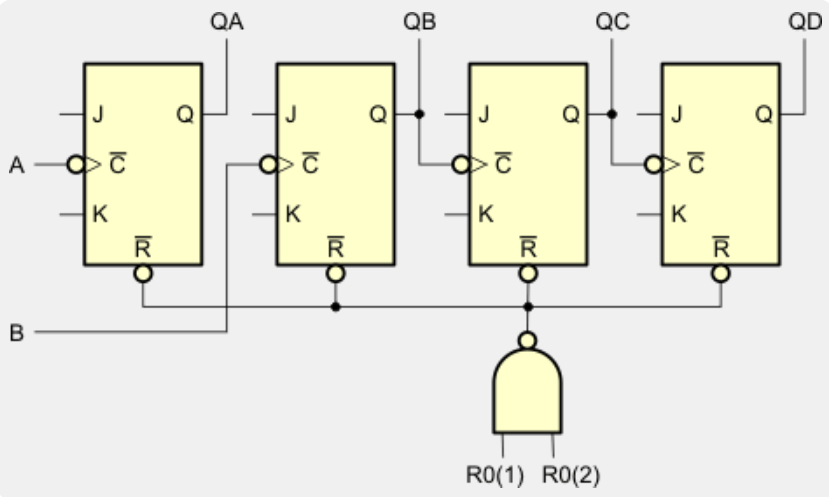
\includegraphics[width=0.7\textwidth]{img/schemes/logic_scheme_7943.png}
            \caption{Schemat logiczny 7493}
            \label{licznik_mod10:schemat_logiczny}
        \end{figure}
    \item Chcąc otrzymać licznik mod 10 należało dodatkowo zadbać o poprawne wywoływanie resetu ($\overline{R}$ na schemacie logicznym (\ref{licznik_mod10:schemat_logiczny})).
    \item Reset powinien następować gdy dostaniemy sekwencję $(1010)_2$ = $(10)_{10}$. Należy wtedy zagwarantować że bramka NAND (patrz: \ref{licznik_mod10:schemat_logiczny}) na swoim wyjściu wygeneruje logiczne \textbf{0} (patrz: \ref{tabela_prawdy:NAND})). Zanegowany sygnał spowoduje reset przerzutników.
    \item Wyjścia licznika QB oraz QD (2 oraz 4 bit) podpięto do bramki NAND (piny 2,3) generującej reset przerzutników.
    \item Wyjścia licznika (QA, QB, QC, QD) zostały wyprowadzone do diod elektroluminescencyjnych     znajdujących się na prawej stronie płytki.
    \item Do wejścia A (pin 14) wpięto sygnał z generatora funkcyjnego o wartościach:
        \begin{center}
            f = 3Hz \\
            $U_{low}$ = 0V \\
            $U_{high}$ = 5V
        \end{center}
    \item LSB (least significant bit) podpięty jest pod pierwszą diodę od lewej (wyjście QA).
        \begin{figure}[H]
            \centering
            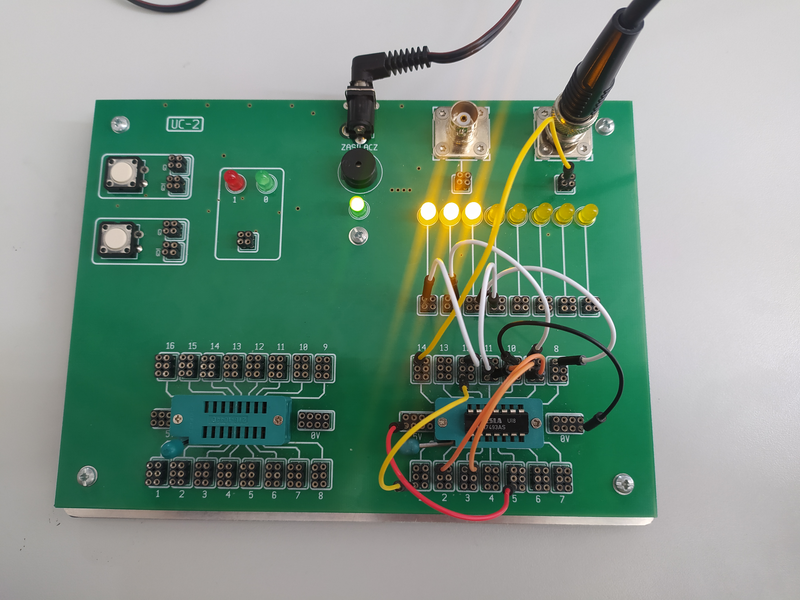
\includegraphics[width=0.7\textwidth]{img/mod10/1653500524710_scaled.png}
            \caption{Zbudowany układ wskazujący $(1110)_2 = (7)_{10}$}
            \label{licznik_mod10:zbudowany_uklad}
        \end{figure}
        
        \begin{figure}[H]
            \centering
            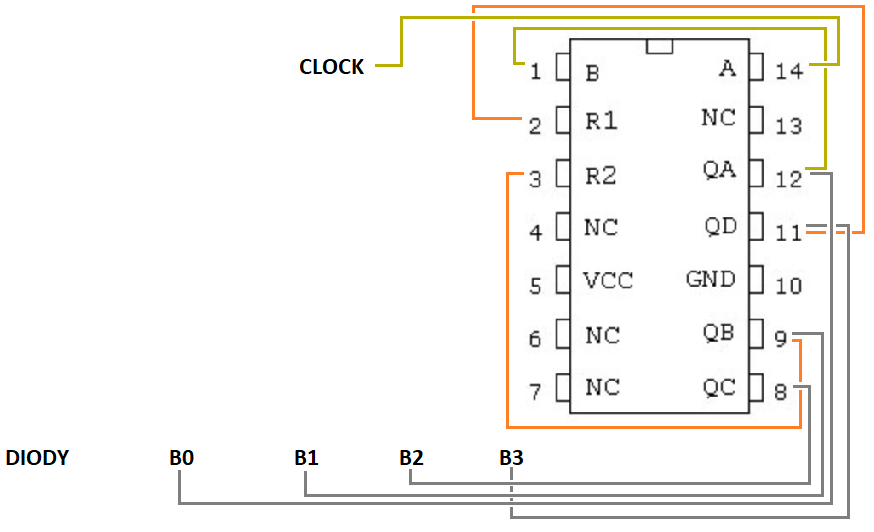
\includegraphics[width=\textwidth]{img/schemes_w_pins/mod10_w_pins.png}
            \caption{Schemat z połączonymi pinami}
            \label{licznik_mod10:schemat_z_pinami}
        \end{figure}
        
    \item Licznik działał \textbf{poprawnie}. Po sekwencji $(1001)_2 = (9)_{10}$ licznik resetował stan do $(0000)_2 = (0)_{10}$. Wciśnięcie impulsatora powodowało reset aktualnego stanu licznika do stanu wyzerowanego $(0000)_2$.
\end{itemize}